% !TeX document-id = {2870843d-1baa-4f6a-bd0a-a5c796104a32}
% !BIB TS-program = biber
% !TeX encoding = UTF-8
% TU Delft beamer template
%pour un ratio 4:3 mettre 43 pour 16:9 169 ; 16:10 1610 ; 
\documentclass[aspectratio=169]{beamer}
\usepackage[french]{babel}
\usepackage[T1]{fontenc} %pour le guillemts à la francaise et ...

%\usepackage{csquotes}
%\usepackage{calc}
\usepackage[absolute,overlay]{textpos}
%\usepackage{graphicx}
%\usepackage{subfig}
%\usepackage{mathtools}
%\usepackage{amsfonts}
%\usepackage{amsthm}
%\usepackage{comment}
%\usepackage{siunitx}
%\usepackage{MnSymbol,wasysym}
%\usepackage{array}
%\usepackage{qrcode}
\usepackage[most]{tcolorbox}
\usepackage{newverbs}
\usepackage{minted}

\setbeamertemplate{navigation symbols}{} % remove navigation symbols
\mode<presentation>{\usetheme[verticalbar=false]{tud}}


\setbeamerfont{footnote}{size=\tiny}
\renewcommand{\cite}[1]{\footnote<.->[frame]{\fullcite{#1}}}
\setlength{\TPHorizModule}{\paperwidth}
\setlength{\TPVertModule}{\paperheight}

\newcommand{\absimage}[4][0.5,0.5]{%
	\begin{textblock}{#3}%width
		[#1]% alignment anchor within image (centered by default)
		(#2)% position on the page (origin is top left)
		\includegraphics[width=#3\paperwidth]{#4}%
\end{textblock}}


\newcommand{\mininomen}[2][1]{{\let\thefootnote\relax%
	\footnotetext{\begin{tabular}{*{#1}{@{\!}>{\centering\arraybackslash}p{1em}@{\;}p{\textwidth/#1-2em}}}%
	#2\end{tabular}}}}

\newverbcommand{\code}{$}{$}
\newcommand{\ang}[1]{<<#1>>}


\title[]{Nextcloud dans la région\\
\ \\
Centre - Val de Loire}
\institute[]{Gip Recia}
\author{Grégory Brousse \and  Pierre Legay}
%\date{}
\setbeamertemplate{itemize subitem}[ball]

\newcommand{\smallsec}{}
\let\oldsection\section
\renewcommand{\section}[1]{\oldsection{#1}\renewcommand{\smallsec}{{\small #1}}}

\newcommand{\sub}{}
\let\oldsubsection\subsection
\renewcommand{\subsection}[1]{\oldsubsection{#1}\renewcommand{\sub}{\smallsec\,: #1}}

\begin{document}
{
\setbeamertemplate{footline}{\usebeamertemplate*{minimal footline}}
\frame{\titlepage \absimage{.10, .20}{.30}{GIP_RECIA.pdf}}
}


\begin{frame}<beamer>{} 
%\tableofcontents[current]
\tableofcontents
\end{frame}



\section{Contexte}
\subsection{Le GIP Recia}

 \begin{frame}{\sub}
	Le Groupement d’Intérêt Public Recia (Région Centre Interactive) associe : 
\begin{itemize}
\item l’État (rectorat) ;
\item plus de 500 structures publiques sur toute la Région Centre Val de Loire ;
\item les Conseils départementaux :
	\begin{itemize}
		\item du Cher ;
		\item de l’Indre-et-Loire ;
		\item de l’Eure-et-Loir ;
		\item de l'Indre ;
		\item du Loir-et-Cher ;
		\item et du Loiret
	\end{itemize}
\item les Universités de Tours et d’Orléans ;
\item l’INSA Bourge ;
\item le CROUS ;
\item Ciclic Centre-Val de Loire ; 
\item GIP e-santé Centre Val de Loire ; 
\item des communes et communautés de communes.
\end{itemize}

\end{frame}

\begin{frame}{\smallsec: Les activités du GIP Recia }
\begin{itemize}
\item Le réseau régional haut débit (renater ReCOR) ;
\item L’hébergement de données ;
\item Aménagement numérique du territoire (conseil / réseaux d’initiative publique) ;
\item Études, expertises, assistance, conseil, veille, animation, observatoire ;
\item Économie numérique et programme transition numérique ;
\item La maintenance informatique des Lycées, des collèges, des CFA, des EFSS ;
\item Les ENT $1^{er}$ et $2^{nd}$ degrés.
\end{itemize}
\end{frame}

\subsection{Les ENT des lycées et collèges de la région}
\begin{frame}{\sub}

ENT du $2^{nd}$ degrés de la région centre.

\begin{itemize}
\item multi-domaines :
	\begin{list}{}{}
		\item ENT des Lycées de la région ;
		\item 1 ENT par départements de la région pour les collèges (6) ;
		\item 238 collèges + 101 lycées + ... 
	\end{list}
	
\item Nombreux utilisateurs potentiels :
\begin{list}{}{}
		 \item $187\,000 $ comptes actifs ; 
		 \item $192\,000$ Élèves ;
		 \item $16\,700$ Enseignants
\end{list}
\item  $61\,000$ Groupes: classe, groupe pédagogique, matière ...  
\item authentification CAS.
\end{itemize}

\end{frame}

\subsection{L'environnement applicatif}
\begin{frame}{\sub}
Infrastructure de production hébergé \raisebox{-2pt}{
\includegraphics[scale=0.1]{aquaray.png}} {\tiny(www.aquaray.com)}.
\begin{itemize}
	\item OpenLdap ;
	\item ENT uPortal ;
	\item Authentification SSO CAS ;
	\item Grouper ;
	\item OnlyOffice ;
	\item Collabora .
	
\end{itemize}
\end{frame}


\section{Infrastructure Nextcloud}
\subsection{L'architecture}
\begin{frame}{L'architecture}
\vspace{-54pt}
\begin{figure}
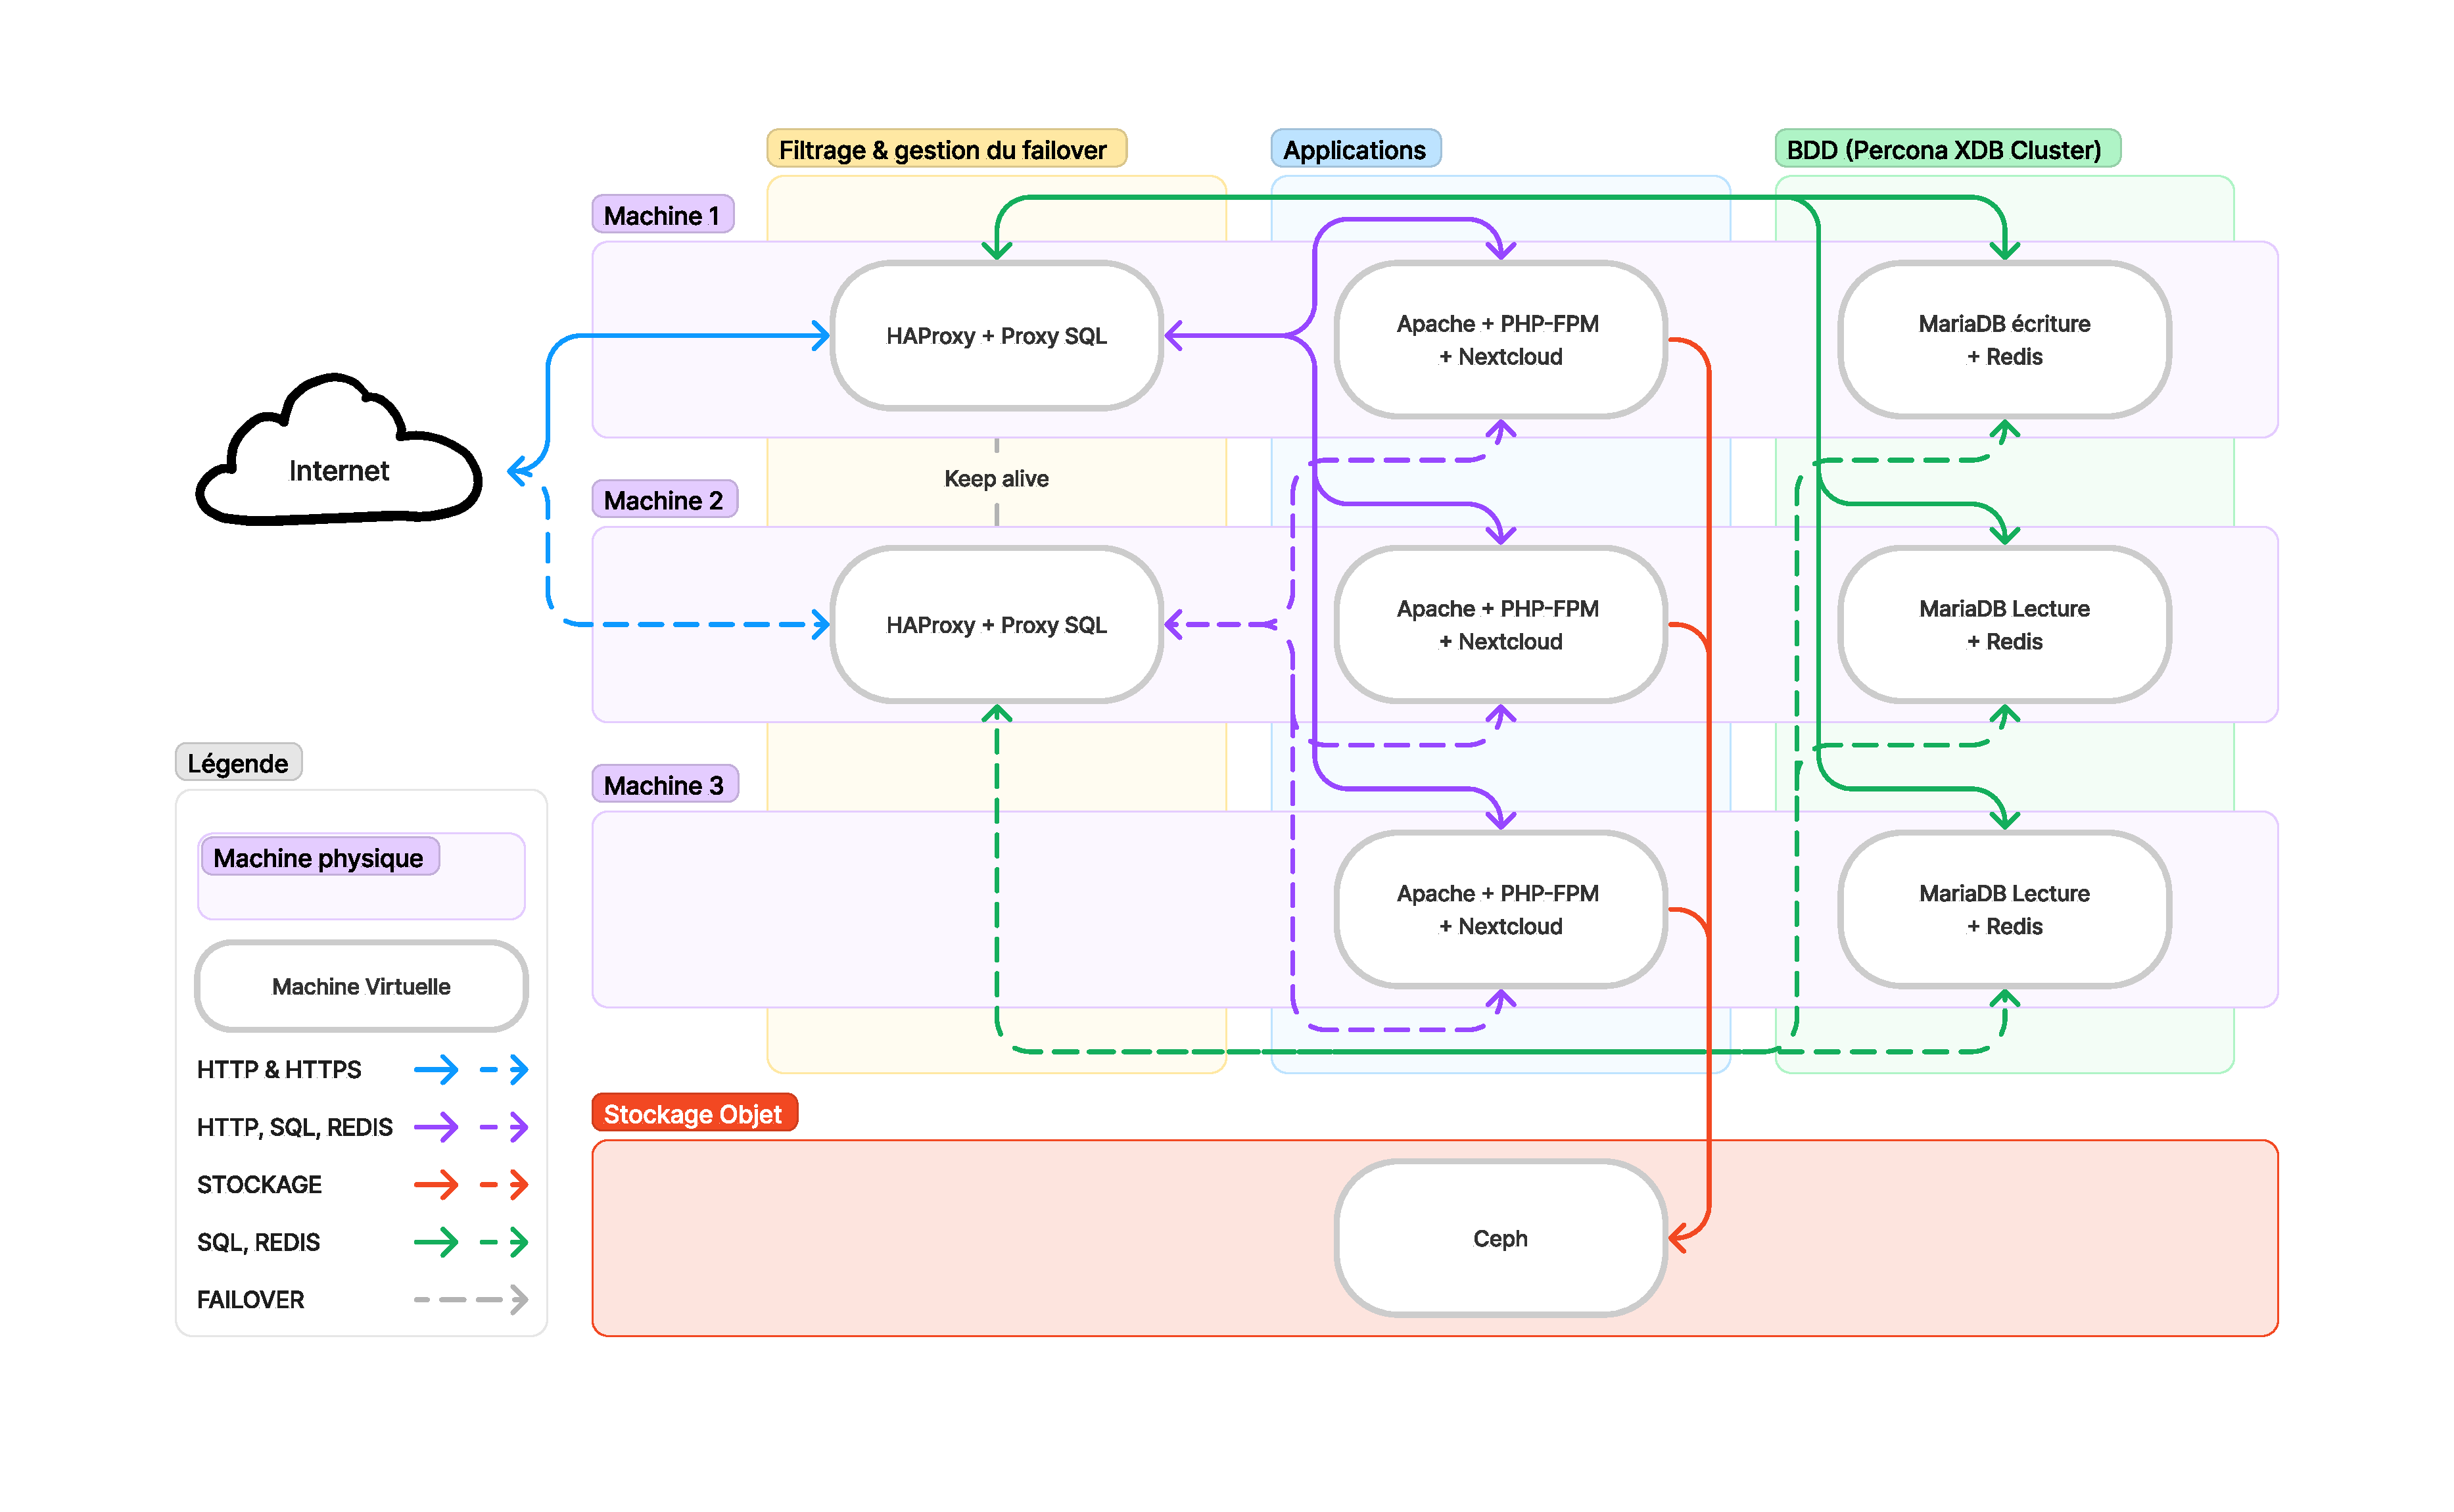
\includegraphics[scale=0.25]{202306-architecture-nextcloud.pdf}
\end{figure}
\end{frame}

\subsection{Les instances de production}
\begin{frame}{Les instances de production} 
Deux instances de production sur la même infrastructure.
\begin{enumerate}
	\item Pour l'ENT depuis mai 2020 (V18.0.3 ... V24.0.12)
		\begin{list}{-}{}
		  \item $9$ domaines (avec leurs CSS) ;
		  \item $372$ établissements ;
		  \item $118\,224$ comptes actifs ;
		  \item $67\,383$ groupes ;
		  \item Création des comptes et groupes automatique depuis LDAP.
		 \end{list}

	\item Pour le GIP Recia (V25.0.6) (extension aux collectivités locales ?) 
	   \begin{list}{-}{}
	   \item Stockage NetApp ;
	   \item Création  automatique des comptes, groupes et  groupFolder.
	   \end{list}
\end{enumerate}
\end{frame}

\section{Nos Adaptations}
\subsection{Plugin cssJsLoader}
\begin{frame}[fragile]{Plugin cssJsLoader}{(steamulo)}
\begin{itemize}
\item Permet de charger nos propres js et css.
\item Personnalisation en fonction du domaine de connexion.
\item Jusqu'en 2022 intégration en \code/iframe/ dans le portail avec \code/postMessage_resize_iframe_in_parent.js/.
\item Depuis 2022 plus d'\code/iframe/, peut-être remplacé par l'utilisation de thème? 
\end{itemize}
\end{frame} 

\subsection{Plugin ladpimporter}
\begin{frame}{Plugin ldapimporter}{(steamulo)} % some commands, e.g. \verb require [fragile]
\begin{itemize}
\item Est dérivé du plugin ``CAS user and group backend'' de Felix Rupp.
\item Permet l'importation des comptes à partir du ldap
\item Fait l'association des comptes et des groupes aux établissements;
		{\small $$ => table\ etablissement $$} 
\item Filtre et traduit les groupes Grouper en groupes Nextcloud
		{\small $$ => table\ asso\_uai\_user\_group $$ } 
\item Gère les quotas des utilisateurs en fonction des leurs groupes.
\end{itemize}
\end{frame}


\begin{frame}{Plugin ldapimporter} % some commands, e.g. \verb require [fragile]
\begin{figure}
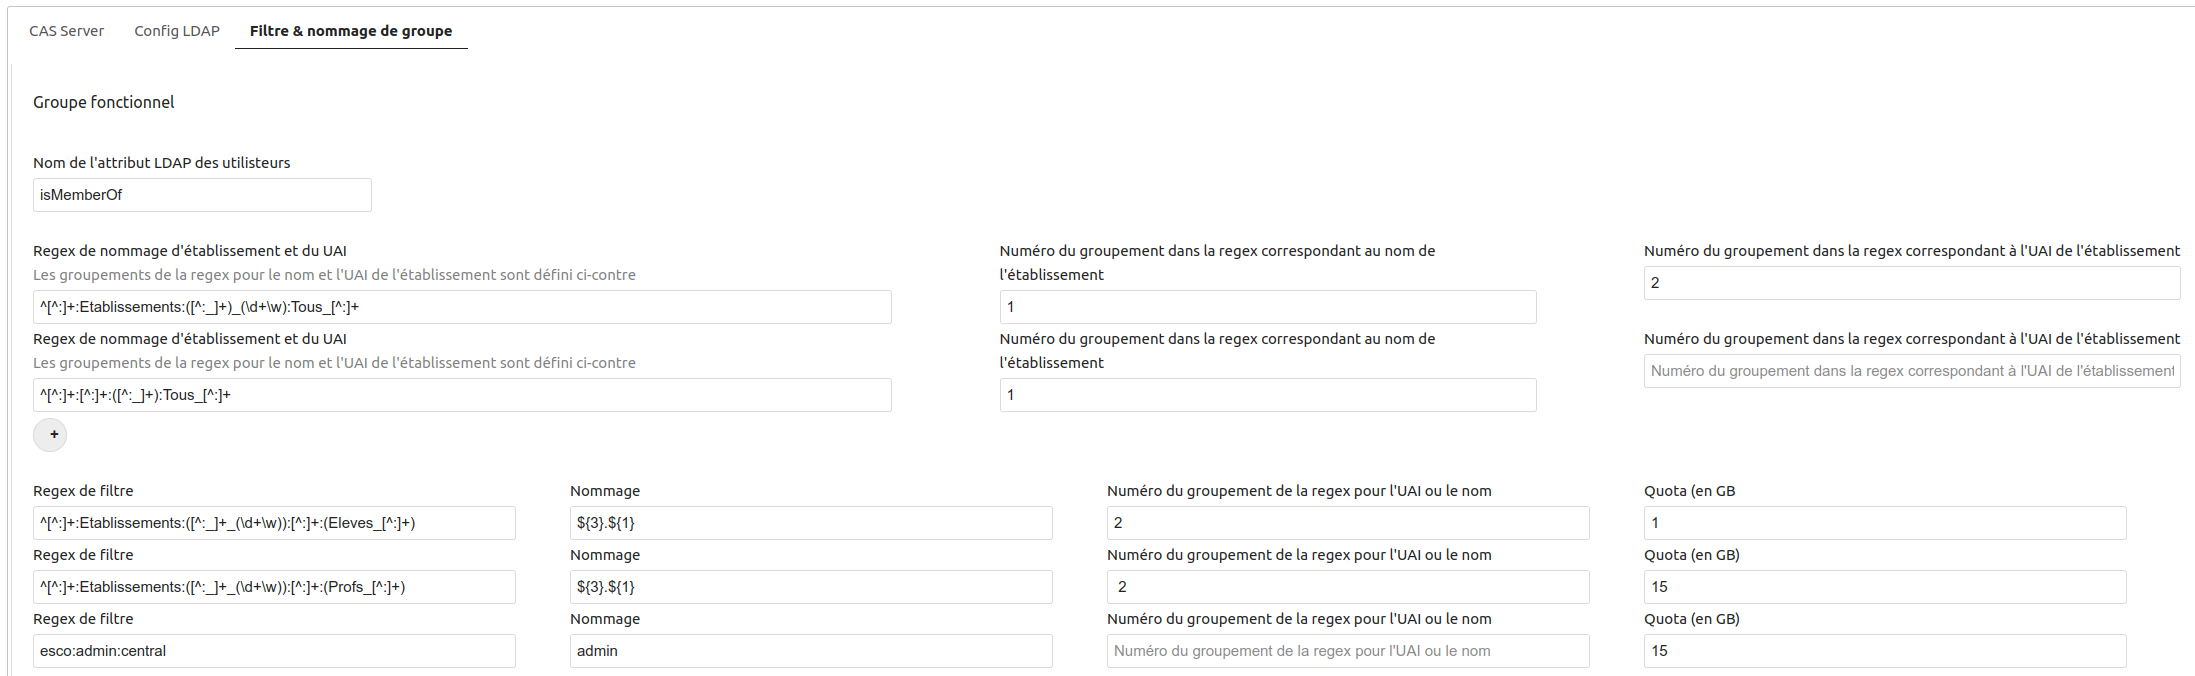
\includegraphics[width=\textwidth, height=0.85\textheight]{ldapimporter.png}
\end{figure}
\end{frame}

\begin{frame}[fragile]{Plugin ldapimporter} % some commands, e.g. \verb require [fragile]
{exemple de filtrage et renommage de groupe}
\begin{list}{}{}
	\item {\tiny Le groupe Grouper :}
\begin{verbatim}
     clg18:Etablissements:ALBERT CAMUS_0180592W:3EME:Eleves_3-2
\end{verbatim}
\item {\tiny satisfait la regex:}
\begin{verbatim}
    ^[^:]+:Etablissements:([^:_]+_(\d+\w)):[^:]+:(Eleves_[^:]+) 
    |   ${3}.${1}  |  2
\end{verbatim}
\item {\tiny est réécrit pour Nexcloud en:}
\begin{verbatim}
    Eleves_3-2.ALBERT CAMUS_0180592W
\end{verbatim}
\item {\tiny et déduit l’appartenance de l'utilisateur à l'établissement}
\begin{verbatim}
    ALBERT CAMUS_0180592W
\end{verbatim}
\end{list}
\end{frame}


\subsection{Plugin files\_sharing}
\begin{frame}[fragile]{Plugin files\_sharing}{Présentation}

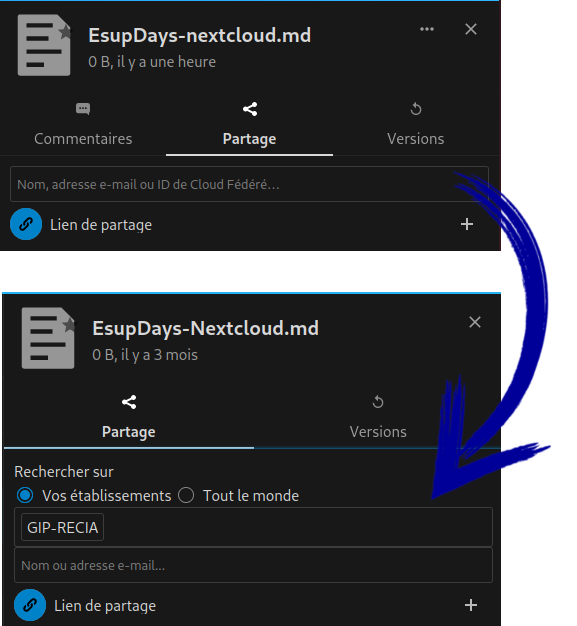
\includegraphics[height=0.75\textheight]{filesharing.png}
\raisebox{3cm}{
\begin{minipage}{8.5cm}
\begin{itemize}
\item Facilité la recherche d'utilisateurs et de groupes pour le partage en permettant la recherche par établissement
\item Fork de l'App File\_sharing de Nextcloud
\item Backend PHP \& frontend Vue JS
\end{itemize}
\end{minipage}
}
\end{frame}

\begin{frame}[fragile]{Plugin files\_sharing}{Utilisation}
\vspace{-20pt}
\begin{figure}
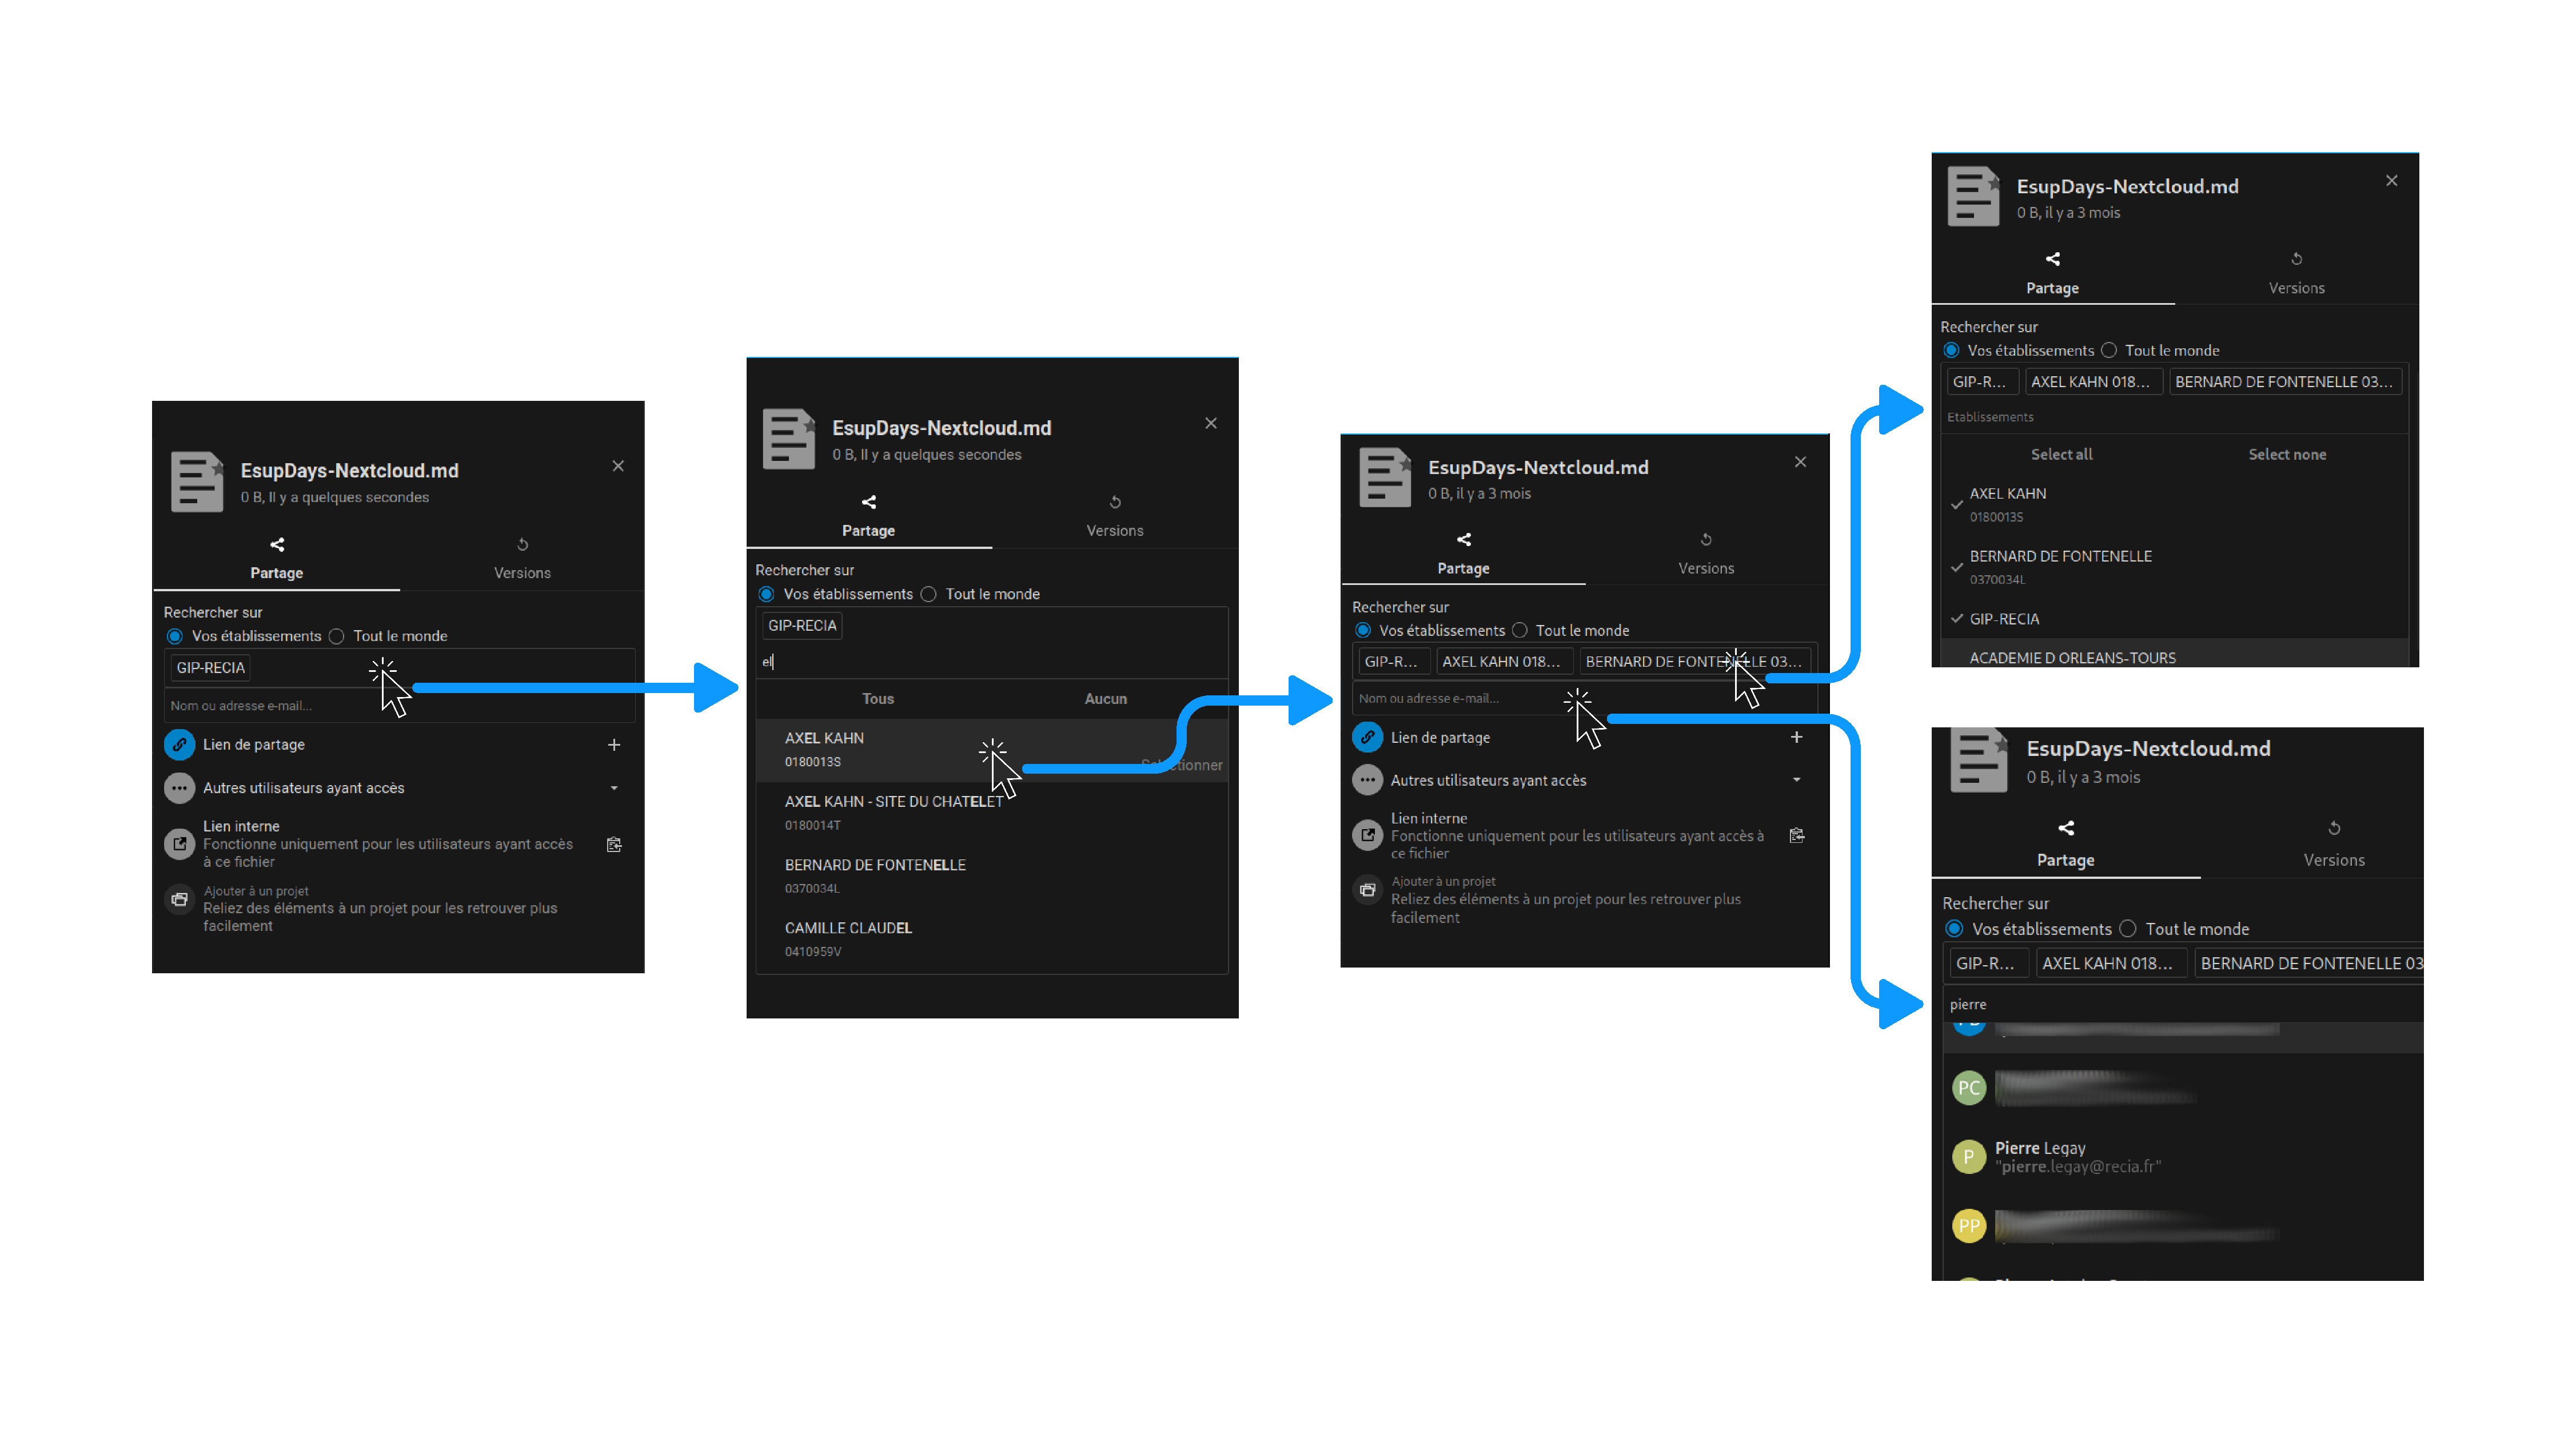
\includegraphics[width=\textwidth]{Fonctionnement-fork-files_sharing.pdf}
\end{figure}
\end{frame}
\begin{frame}[fragile]{Plugin files\_sharing}{Backend}
\begin{itemize}
	\item 2 routes :
		\begin{list}{-}{}
		\item recherche d'établissements liés à l'utilisateur courant
		\item recherche des utilisateurs \& groupes liés à un établissement
		\end{list}
	\item 1 contrôleur
\end{itemize}

\end{frame}

\begin{frame}[fragile]{Plugin files\_sharing}{Frontend}

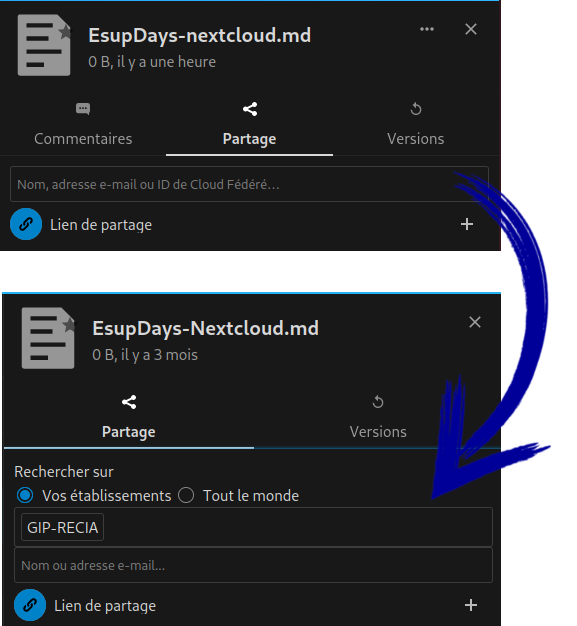
\includegraphics[height=0.75\textheight]{filesharing.png}
\raisebox{3cm}{
\begin{minipage}{8.5cm}
Remplacement dans la vue $SharingTab$ du composant $SharingInput$ par :
\begin{itemize}
\item boutons radios de sélection du type de recherche
\item composant de recherche d'établissement basé sur le composant $NcMultiselect$ 

\item composant dérivé du composant originel $SharingInput$
\end{itemize}
\end{minipage}
}
\end{frame}

\subsection{Bandeau ENT}
\begin{frame}{Bandeau ENT}
Les navigateurs n'acceptant plus le cross-domaine sur les cookies de session (auth CAS).
\begin{itemize}
	\item Création d'un composant web simulant le portail (à la prolongation\_ent)
	\item Intégration dans NC via un thème.
	\item tenant compte du multi-domaines   
\end{itemize}
\end{frame}


\section{Les difficultés rencontrées}
\subsection{Stockage Objet}
\subsection{UI groupes et intégration ENT}
\begin{frame}[fragile]{Les difficultés rencontrées}
\begin{itemize}

\item Le stockage object (en \small{V18});  OpenIo recommandation de ne pas dépasser $500\,000$ objets par \ang{bucket}. Obligation des sortir les \ang{avatars} \ang{previews} du \ang{bucket} par défauts. (Résolut pour les \ang{previews} dans les versions récentes \code/objectstore.multibucket.preview-distribution/).

\item Avec le stockage object pas de \ang{snapshot}, comment se prémunir d'une attaque de type \ang{ransomware} ; projet a l'étude avec Arawa. 

\end{itemize}


\begin{itemize}
\pause \item Le grand nombre de groupes génère un \ang{time out} à l'appel de la gestions des utilisateurs (pas de pagination sur les groupes)
\pause \item Ajout du bandeau \ang{header} et \ang{footer} pause difficultés. 
\end{itemize}

\end{frame}



%\begin{frame}[fragile]{Historique}
%\begin{itemize}
%\item Premier déploiement avec établissements de test en mai 2020 version 18.0.3 
%\item Généralisation à tous les établissement à partir de Septembre 2020 par groupes d'une dizaine d'établissements. 
%\item Intégration dans le portail en mode \code/iframe/.
%\end{itemize}
%\end{frame}


\end{document}

